\section{Filtros digitales del giroscopio}
\label{sec:filtros}

\subsection{Dónde están y qué filtran}

La señal de tasa que llega al PID es la salida del estimador de actitud
(giroscopio menos sesgo estimado) pasada por una cadena de filtros por eje
(\cod{Simulation.step\_control}). Por defecto la cadena tiene dos etapas:
la etapa 0 es un pasa-bajos \val{filtroDef} y la etapa 1, un notch centrado en
177~Hz con $Q=\val{notchQ}$ que viene \val{notchDef}. El corte de
\val{filtroDefFc}~Hz (la 2.ª edición y las primeras versiones de este núcleo
usaban 80~Hz) se fijó junto con el derivativo del lazo de tasa a partir del
barrido conjunto de la \cref{sec:barridos}: un corte más bajo quita más
vibración y su retardo adicional lo compensa el adelanto de fase de un $k_d$
mayor (\cref{sec:control}). El estimador de actitud recibe el giroscopio
sin filtrar, como en PX4, porque integra la tasa y la integral de un tono de
177~Hz es despreciable. El \emph{acelerómetro}, en cambio, sí se filtra antes
del estimador, con un Butterworth de \val{accLpf}~Hz
(\cod{SimConfig.ahrs\_accel\_lpf\_hz}), por la razón no lineal que explica
la \cref{sec:estimadores}.

Todo filtro introduce retardo. El compromiso que el usuario debe resolver,
y que los barridos automáticos de la \cref{sec:barridos} cuantifican, es
cuánto ruido quitar a cambio de cuánto margen de fase perder en el lazo de
tasa.

\subsection{El biquad}

Todos los tipos son secciones de segundo orden (\emph{biquad}) en forma
directa II transpuesta, con los coeficientes del \emph{Audio EQ Cookbook} de
Bristow-Johnson \cite{rbj}, que corresponden a la transformación bilineal
con la frecuencia de corte pre-distorsionada. Es el mismo filtro de
Betaflight y PX4 sobre el giroscopio. La ecuación en diferencias
(\cod{Biquad.process}) es
\begin{equation}
y_k = b_0x_k + z_1,\qquad
z_1 \leftarrow b_1x_k - a_1y_k + z_2,\qquad
z_2 \leftarrow b_2x_k - a_2y_k ,
\label{eq:df2t}
\end{equation}
con $H(z)=\dfrac{b_0+b_1z^{-1}+b_2z^{-2}}{1+a_1z^{-1}+a_2z^{-2}}$. Llamando
$\omega_0=2\pi f_c/f_s$ y $\alpha=\sin\omega_0/(2Q)$, y normalizando por
$a_0=1+\alpha$:
\begin{align}
\text{común:}\quad & a_1=\tfrac{-2\cos\omega_0}{a_0},\qquad a_2=\tfrac{1-\alpha}{a_0};\nonumber\\
\text{pasa-bajos:}\quad & b_0=b_2=\tfrac{1-\cos\omega_0}{2a_0},\qquad b_1=\tfrac{1-\cos\omega_0}{a_0};\label{eq:lpf}\\
\text{notch:}\quad & b_0=b_2=\tfrac{1}{a_0},\qquad b_1=\tfrac{-2\cos\omega_0}{a_0}.\label{eq:notch}
\end{align}

\paragraph{Tipos.} \textbf{Butterworth} es el pasa-bajos con $Q=1/\sqrt2$
(máximamente plano). \textbf{Pasa-bajos} deja libre el $Q$: con $Q>0.707$
el filtro tiene un pico antes del corte pero menos retardo en la banda de
paso. \textbf{Chebyshev~I} de orden 2 con rizado $r_p$~dB: con
$\varepsilon=\sqrt{10^{r_p/10}-1}$ y $v_0=\operatorname{asinh}(1/\varepsilon)/2$,
el polo analógico normalizado es
$s=-\sinh v_0\sin\frac{\pi}{4}\pm j\cosh v_0\cos\frac{\pi}{4}$; de su módulo
$\omega_n$ y su parte real se obtienen $Q=\omega_n/(2|\Re s|)$ y la frecuencia
de diseño $f_c\,\omega_n$, y con ellas se usa \eqref{eq:lpf}. Para 1~dB
resulta $Q=\val{chQ}$. El código normaliza la ganancia continua a 0~dB (la
verificación da 0.0~dB en continua y un máximo de $+1.0$~dB en la banda de
paso): el rizado queda \emph{por encima} de la
ganancia unitaria, a diferencia del Chebyshev de libro de orden par, que
tiene $-r_p$~dB en continua. \textbf{Notch} rechaza una banda angosta
alrededor de $f_c$, tanto más angosta cuanto mayor es $Q$.

\paragraph{Detalles de robustez.} $f_c$ se acota a $0.98$ veces Nyquist y
$Q\ge0.05$; \cod{reset(x0)} inicializa el estado en el régimen permanente de
una entrada constante (sin transitorio de arranque); \cod{Simulation.set\_filter},
que rediseña un filtro en pleno vuelo (desde la GUI o un barrido), lo reinicia
así con la tasa actual, para que el cambio no produzca un escalón en la
señal; si la salida no es finita, el filtro se reinicia y deja pasar la
entrada.

\subsection{Compromiso atenuación--retardo}

La \cref{tab:filtros} y la \cref{fig:bode} comparan, a $f_s=500$~Hz, el
retardo de grupo en 10~Hz (la zona donde vive la dinámica del lazo de tasa)
con la atenuación en la frecuencia de paso de pala.

\begin{table}[H]
\centering
\small
\caption{Retardo y atenuación de los filtros (calculados de la respuesta en
frecuencia exacta de cada biquad, \cod{Biquad.response}).}
\label{tab:filtros}
\begin{tabular}{lccc}
\toprule
Filtro & Retardo de grupo & Fase & Atenuación \\
 & a 10~Hz [ms] & a 10~Hz [$^\circ$] & a 177~Hz [dB] \\
\midrule
Butterworth 80~Hz & \val{gdBWo} & \val{phBWo} & \val{atBWo} \\
Butterworth 60~Hz & \val{gdBWs} & \val{phBWs} & \val{atBWs} \\
Pasa-bajos 40~Hz, $Q=0.707$ & \val{gdLPc} & \val{phLPc} & \val{atLPc} \\
Chebyshev~I 80~Hz, 1~dB & \val{gdCH} & \val{phCH} & \val{atCH} \\
Notch 177~Hz, $Q=4$ & \val{gdNO} & \val{phNO} & $<-200$ (cero exacto) \\
\bottomrule
\end{tabular}
\end{table}

\begin{figure}[H]
\centering
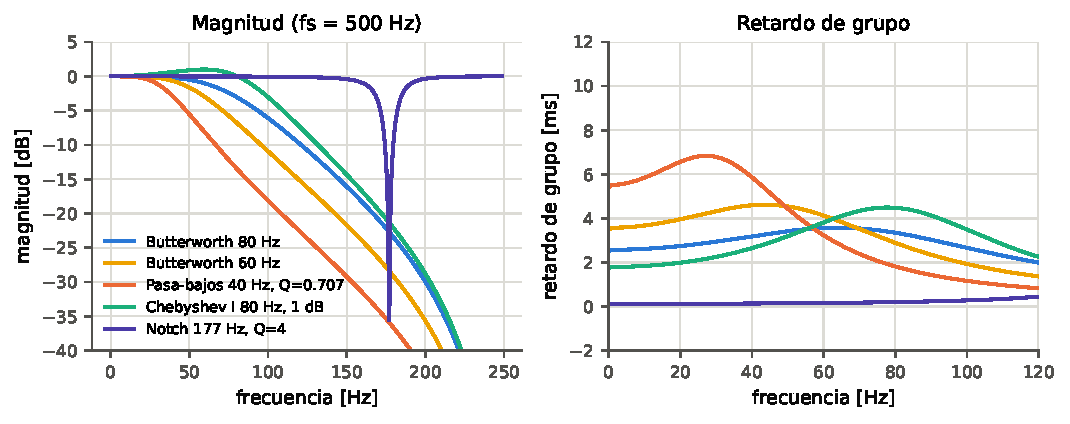
\includegraphics[width=\textwidth]{filtros_bode.pdf}
\caption{Magnitud y retardo de grupo de los filtros de la \cref{tab:filtros}.}
\label{fig:bode}
\end{figure}

Bajar el corte de 80 a 60~Hz gana 6~dB de atenuación de la vibración a
cambio de 1~ms de retardo; bajarlo a 40~Hz gana 13~dB y duplica el retardo. El notch, en cambio, anula el tono con un retardo más de diez
veces menor que cualquier pasa-bajos, pero solo si está centrado: en la
\cref{sec:barridos} se mide que un notch angosto descentrado 2~Hz pierde casi
todo su beneficio, y el tono se mueve con el acelerador
(\cref{sec:vibracion}).

\subsection{Filtro de primer orden}

El término derivativo del PID usa un filtro de primer orden discreto
(\cod{control/pid.py}, y la clase \cod{PT1} de \cod{filters.py}):
\begin{equation}
y_k = y_{k-1}+\alpha\,(x_k-y_{k-1}),\qquad \alpha=\frac{\Delta t}{\tau+\Delta t},\quad \tau=\frac{1}{2\pi f_c}.
\label{eq:pt1}
\end{equation}
